\documentclass{article}
\usepackage[dblblindworkshop]{neurips_2026}
\workshoptitle{Who Verifies the Agents? Toward Reliable Agent Development}
\usepackage{amsmath,amssymb,amsthm,booktabs,tabularx,array}
\usepackage{tikz}
\usetikzlibrary{arrows.meta,positioning,shapes.geometric,fit}
\usepackage[colorlinks=true,allcolors=blue]{hyperref}
\usepackage[nameinlink,noabbrev]{cleveref}
\newtheorem{theorem}{Theorem}
\newcommand{\Reach}{\operatorname{Reach}}
\title{Verification-Gated Hierarchical Execution: A Demo for Long-Horizon Agents}
\author{Anonymous Author(s)}

\begin{document}
\maketitle

\begin{abstract}
Long-horizon agents can fail after many locally plausible steps: a completion is unsupported, an intermediate artifact becomes stale, or a repair silently invalidates downstream work. Post-hoc scoring identifies some failures but leaves execution control unresolved: what was checked, what evidence supports it, and where should execution resume? We present a runnable, package-resident agent harness in which persistent intent is refined through \emph{Goal $\to$ Plan $\to$ Phase $\to$ durable intent contract (DIC) $\to$ disposable execution prompt stack (EPS) $\to$ Prompt/Run $\to$ Action}, actions bind to evidence, and verification is a control signal with four outcomes: accept, repair, replan, or escalate. The implementation records recoverable lineage and lets a failed phase instantiate a new bounded execution stack while preserving its durable contract. In a deterministic worked demo, a failed producer is repaired; its changed output invalidates four declared downstream nodes; two unaffected nodes retain prior evidence; and re-verification accepts the repaired run. Fresh-store recovery reconstructs and validates the persisted hierarchy. Under complete dependency declarations and version-bound evidence, a compact locality theorem characterizes when unaffected work can be safely retained. The demonstrated results show how evidence-gated verification can serve as a closed-loop control mechanism for bounded recovery in long-horizon agent execution.
\end{abstract}

\section{Verification as execution control}
Agent loops already interleave reasoning, tool use, planning, and feedback \citep{yao2023react,shinn2023reflexion,zhou2024lats}. The verification problem becomes different when a run spans many artifacts and contexts. A late ``wrong'' leaves unanswered: \emph{what exactly was checked, which evidence supported it, which later artifacts depended on it, and whether the next action is a retry, an upward replan, or a human escalation?} Full restart is safe but wasteful; local retry is efficient but unsafe if hidden dependencies exist. Reliability evaluation also shows that tool-using agents can fail in ways that require environment-grounded checks rather than self-assessment alone \citep{debenedetti2024agentdojo}.

We treat verification as an execution-time state transition, drawing on runtime-monitoring ideas \citep{leucker2009runtime}. \Cref{fig:architecture} summarizes the implemented object. The central contribution is the joint execution contract: persistent intent, bounded refinement, evidence lineage, explicit verification outcomes, and an inspectable recovery scope that survives fresh-session recovery.

\begin{figure}[t]
\centering
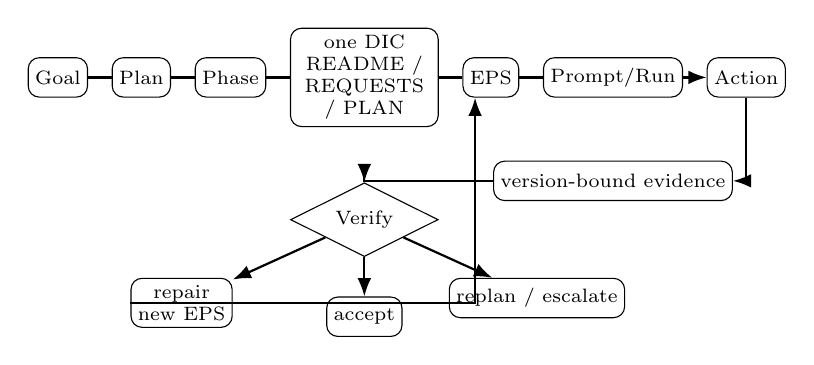
\begin{tikzpicture}[font=\scriptsize,>=Latex,node distance=3.0mm and 3.0mm,
 box/.style={draw,rounded corners,inner sep=2.5pt,align=center,minimum height=5mm},
 flow/.style={-Latex,thick}]
\node[box] (goal) {Goal};
\node[box,right=of goal] (plan) {Plan};
\node[box,right=of plan] (phase) {Phase};
\node[box,right=of phase,text width=17mm] (dic) {one DIC\\README / REQUESTS / PLAN};
\node[box,right=of dic] (eps) {EPS};
\node[box,right=of eps] (run) {Prompt/Run};
\node[box,right=of run] (act) {Action};
\node[box,below=8mm of run] (ev) {version-bound evidence};
\node[diamond,draw,aspect=2,below=7mm of dic] (ver) {Verify};
\node[box,below left=5mm and 12mm of ver] (repair) {repair\\new EPS};
\node[box,below=5mm of ver] (accept) {accept};
\node[box,below right=5mm and 6mm of ver] (up) {replan / escalate};
\draw[flow] (goal)--(plan)--(phase)--(dic)--(eps)--(run)--(act);
\draw[flow] (act)|-(ev);
\draw[flow] (ev)-|(ver);
\draw[flow] (ver)--(repair);
\draw[flow] (ver)--(accept);
\draw[flow] (ver)--(up);
\draw[flow] (repair.west) -| ([xshift=-2mm]eps.south);
\end{tikzpicture}
\caption{Implemented control surface. The DIC is the persistent multi-view Phase contract; an EPS is a disposable, state-specific realization. Evidence returns through a verification gate that changes execution rather than merely scoring a finished run.}
\label{fig:architecture}
\end{figure}

\paragraph{Implemented control surface.}
The supplied Python runtime uses package-local \texttt{STATE.json} under \texttt{.ai-workflow/} as the authority index and JSON/Markdown records under \texttt{runtime/}. Every Action is linked to its EPS, DIC, Phase, Plan, prompt node, result, and evidence paths. Evidence paths are indexed back to the producing action. A recovery routine reconstructs and validates lineage from package state without relying on the conversation that produced it.

\section{Persistent contract, disposable execution}
A \textbf{Plan} is the approved multi-phase authority surface. A \textbf{Phase} is a coherent milestone inside it. Each Phase has exactly one \textbf{durable intent contract (DIC)} package: complementary views of the same persistent contract, with execution order encoded in \texttt{PLAN.md}. \texttt{README.md} summarizes the Phase; \texttt{REQUESTS.md} records concrete goals and acceptance targets; \texttt{PLAN.md} stores the durable prompt/dependency graph, including parallel subagents, dependencies, merge nodes, and conditional review/repair branches. \texttt{ARCHITECTURE.md} and \texttt{TEST\_MATRIX.md} are materialized when relevant, and user-defined Markdown views are first-class.

A \textbf{disposable execution prompt stack (EPS)} is a just-in-time instantiation of DIC plan nodes for the current state and attempt. It records node dependencies, plan-node identity, executor, prompts/instructions, parallel groups, subagent flags, and stop conditions. Multiple EPS attempts can therefore refine the same DIC after new evidence arrives. This separation preserves durable intent while operational work is regenerated and re-verified.

\paragraph{Four outcomes.}
The runtime records \texttt{accept}, \texttt{repair}, \texttt{replan}, or \texttt{escalate}. \texttt{repair} keeps the Phase active so a new EPS can be generated. \texttt{replan} crosses the approved authority boundary through a protocol-change escalation, while \texttt{escalate} raises a material scientific/authority boundary. Thus a verifier participates in control flow even when it cannot itself repair the artifact.

\section{Worked demo: failure to bounded recovery}
We added a self-contained deterministic driver, \texttt{demo\_trace.py}, that composes two mechanisms already present in the package: the core \texttt{WorkflowStore} hierarchy/evidence/verification runtime and the existing declared-dependency impact-cone helper.

The durable DIC contains seven plan nodes (\Cref{fig:demo}). The first EPS instantiates all seven and records versioned evidence. A deterministic verifier then rejects \texttt{normalize}'s output with a schema/version mismatch and records outcome \texttt{repair}. Repairing that producer changes the declared key \texttt{normalized}; \texttt{experiment} is its direct reader, so the declared downstream cone is \{\texttt{experiment}, \texttt{table}, \texttt{paper}, \texttt{release}\}. The second EPS instantiates the repair source plus those four nodes. \texttt{collect} and the independent \texttt{theory} node are not re-executed. Re-verification records \texttt{accept}, the Phase completes, and a fresh store reports package recovery as valid. The DIC identifier is unchanged across the two EPS attempts.

\begin{figure}[t]
\centering
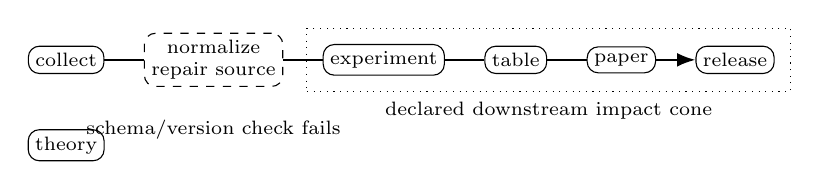
\begin{tikzpicture}[font=\scriptsize,>=Latex,node distance=5.5mm and 5mm,
 box/.style={draw,rounded corners,inner sep=2.5pt,align=center},
 bad/.style={draw,dashed,rounded corners,inner sep=2.5pt,align=center},flow/.style={-Latex,thick}]
\node[box] (c) {collect};
\node[bad,right=of c] (n) {normalize\\repair source};
\node[box,right=of n] (e) {experiment};
\node[box,right=of e] (t) {table};
\node[box,right=of t] (p) {paper};
\node[box,right=of p] (r) {release};
\node[box,below=7mm of c] (th) {theory};
\draw[flow] (c)--(n)--(e)--(t)--(p)--(r);
\node[below=3mm of n,align=center] {schema/version check fails};
\node[draw,dotted,fit=(e)(t)(p)(r),inner sep=2mm,label=below:{declared downstream impact cone}] {};
\end{tikzpicture}
\caption{Deterministic worked demo. Repair changes the \texttt{normalized} key, so the second EPS contains the repair source and four downstream nodes; \texttt{collect} and independent \texttt{theory} evidence are retained. Evidence class: deterministic structural/runtime demonstration.}
\label{fig:demo}
\end{figure}

This trace establishes the demonstrated capability: a verification result changes subsequent execution, preserves inspectable lineage for retained work, and confines re-execution to an explicit declared dependency scope. Its evidence class is deterministic structural/runtime validation.

\section{Why local retention can be sound}
Let the durable execution graph be a DAG $G$. Node $v$ declares a read set $R_v$ and write set $W_v$. After repairing a source changes keys $\Delta$, define the direct readers and downstream impact cone
\[
B(\Delta)=\{v:R_v\cap\Delta\neq\varnothing\},\qquad
\mathcal I(\Delta)=\Reach_G(B(\Delta)).
\]

\begin{theorem}[Dependency-local recovery]
Assume complete declared dependencies/read--write footprints, evidence bound to input and artifact versions, deterministic execution under recorded parameters or fresh re-verification, and no undeclared mutable shared state. After a repair changes only $\Delta$, completed outputs and evidence for every $v\notin\mathcal I(\Delta)$ remain contract-valid; re-execution need only be considered inside $\mathcal I(\Delta)$.
\end{theorem}
\emph{Sketch.} In topological order outside the cone, a node neither reads $\Delta$ nor depends on a changed predecessor; hence its declared inputs and predecessor outputs are unchanged. Its output/evidence therefore remains valid under the assumptions. The result adapts the dependency-locality principle used by incremental build systems \citep{mokhov2018build}; one hidden edge invalidates the guarantee.

\section{Validation, scope, and relation to prior work}
\begin{table}[t]
\caption{Evidence currently present in the package. Categories are intentionally separated.}
\label{tab:evidence}
\centering
\small
\begin{tabularx}{\linewidth}{@{}p{0.21\linewidth}p{0.23\linewidth}X@{}}
\toprule
Evidence & Observed result & What it supports \\
\midrule
Package-only recovery & \texttt{ok=true}; clean & persistent-state recovery and lineage checks \\
Deterministic demo & repair $\to$ accept; one DIC, two EPS attempts & structural closed-loop recovery under declared dependencies \\
Locality theorem & proved under explicit assumptions & conditional safety of retaining nodes outside the cone \\
Controlled agent benchmark & frozen protocol; execution pending & planned comparative evaluation \\
\bottomrule
\end{tabularx}
\end{table}

Feedback agents such as Reflexion and search/planning agents such as LATS use external or self-generated feedback to improve later decisions \citep{shinn2023reflexion,zhou2024lats}; automated design work searches over whole agent scaffolds \citep{hu2025adas}. Our systems contribution is the execution-time contract: what persists across attempts, how evidence is attached, and how a verification result chooses a bounded recovery or authority transition. Runtime-verification work motivates monitoring during execution \citep{leucker2009runtime}, while dependency-aware build systems motivate selective recomputation \citep{mokhov2018build}. The distinctive systems object is their composition into a persistent, evidence-gated recovery contract.

\paragraph{Artifact surface and auditability.}
The runnable artifact exposes the state transitions directly. \texttt{demo\_trace.py} builds a fresh temporary package, approves one Plan/Phase/DIC, records evidence-linked Actions for a seven-node EPS, records \texttt{repair}, computes the declared impact cone, executes the five-node repair EPS, records \texttt{accept}, completes the Phase, and reopens the package in a fresh store. \texttt{demo\_trace.json} records the two EPS node sets, stable DIC, outcomes, retained nodes, and recovery result; the anonymous supplement contains the cleaned runtime, DIC/EPS schemas/templates, demo, and relevant verification/recovery tests.

\paragraph{Fresh-session recovery audit.}
Recovery validates Phase dependencies, DIC lineage and required views, the stored DIC hash, required report files, and every EPS--DIC binding. Malformed structures become errors and a legacy single-file DIC becomes a migration warning. Thus \texttt{recovery\_ok=true} certifies structural consistency after reopening the persisted hierarchy; semantic validity remains delegated to verifier evidence.

\paragraph{Verification boundary.}
Evidence pointers establish lineage, while semantic validity remains the verifier's responsibility. Verifier correctness, adversarial robustness of tool outputs, and dependency completeness are external assumptions. The demo explicitly composes the implemented impact-cone helper with \texttt{repair}; automatic impact-cone scheduling remains outside the core runtime.

\paragraph{Planned empirical closure.}
The package freezes an unexecuted comparative protocol spanning direct/reactive execution (C0), flat plan-and-execute (C1), hierarchy without gated recovery (C2), and hierarchy with verification-triggered repair/replanning (C3), with matched-budget controls. Tasks vary dependency structure and injected faults; planned outcomes include unsupported completion, detection latency, downstream propagation, recovery locality, and rework. These remain evaluation commitments, so no comparative numbers appear here.

\paragraph{Limitations.}
Declared read/write dependencies can be incomplete, and the core runtime does not infer them automatically. Verifiers can miss properties absent from their evidence surface; \texttt{independent} is provenance rather than proof of statistical independence. Replanning crosses a material authority boundary, the deterministic demo provides structural rather than confirmatory comparative evidence, and the hierarchy may be unnecessary overhead for short tasks.

\paragraph{Demo takeaway.}
The implemented trace exposes a concrete systems pattern: evidence-bound verification can turn failure into a localized, inspectable state transition with retained work and a bounded recovery scope. Recovery itself therefore becomes an auditable object for long-horizon agent development.

\bibliographystyle{plainnat}
\bibliography{references}
\end{document}
